% kapitel2.tex
\chapter{Fundamentals and Background}
\label{chapter:fundamentals}

As stated in the introduction, most routing algorithms focus on finding shortest paths between two or more points.
Many of those approaches have been reviewed in surveys (see for example \cite{wayahdi_greedy_2021}).
Additionally, there have been many heuristic approaches, like local search variants \cite{braysy_vehicle_2005, irnich_sequential_2006, ropke_heuristic_2005} or different neighborhood-based ideas \cite{braysy_vehicle_2005, irnich_sequential_2006, ropke_heuristic_2005} that offer faster results in exchange for not necessarily finding the single best solution, but only close approximations.
Much research has been done and is still ongoing for these kinds of problems, stemming from the fact that many graph routing problems (for example the \texttt{Traveling Salesman Problem (TSP)} \cite{gendreau_handbook_2010}, the \texttt{Vehicle Routing Problem (VRP)}  \cite{braysy_vehicle_2005, irnich_sequential_2006} or the \texttt{Arc Orienteering Problem (AOP)} \cite{agarwal_correlated_2023, buchin_tour4me_2022}) are NP-hard \cite{reinelt_traveling_2003}.
 
Finding the shortest path is important in various parts of daily life.
Whether the problem is finding the best (shortest, quickest, most convenient) way to commute to work or reach a supermarket by car or bike, or minimize travel time by bus or any other means of transportation.
The examples for shortest path problems are numerous.
Additionally, shortest paths are not limited to real-world networks but can also prove useful for social networks or any form of digital network \cite{potamias_fast_2009}.
Here, different algorithms can help calculate friend networks or support the routing of data through virtual networks. 

\section{Arc Orienteering Problem}
\label{sec:aop}

The \texttt{Arc Orienteering Problem} is a variant of the \texttt{Orienteering Problem (OP)} and forms the central concept for roundtrip generation.
Souffiau et al.\ \cite{souffriau_planning_2011} describe the problem and underlying ideas, as well as basic definitions of the AOP in detail.
While many other variants of the OP mainly use the nodes of a graph to determine the benefit, the AOP focuses specifically on arcs -- the edges -- of the graph.
Here, the underlying question is to generate a path that maximizes the profit of the contained edges while staying within the bounds of a maximum length ($C_{max}$). 
Each edge has a cost $c_{ij}$ and a profit $p_{ij}$, which contribute to the overall length and overall profit of the generated path.
The maximum length has to be defined.
Furthermore, a start- and endpoint have to be determined.
For roundtrips, these two points are defined by the same vertex, so only the starting point $s$ needs to be selected.

In a graph $G=(V,E)$, vertex positions are denoted by $v_{ij}$.
Whether or not an edge is part of a path is given by $\chi_{ij}$.
Based on Souffriau et al. \cite{souffriau_planning_2011}, the objective is to maximize the overall profit, while adhering to several constraints:

First, both the startpoint and the endpoint have to be part of the resulting path, ensuring that the specified start will always be used. 
For roundtrips, this constraint can be simplified to only using the first or the last point of a tour.
Secondly, the resulting tour has to be fully connected.
Otherwise, several independent path fragments could be created without ever resulting in a closed tour.
Additionally, all edges and vertices that are part of the result have to be visited.
Leaving partial paths out and still adding these to the result is not possible.
Furthermore, the resulting length is constrained by a maximum value $C_{max}$.
Lastly, ensuring that no sub-tours are created is another important factor, preventing inner loops from occurring and thus resulting in a single outer loop.

%\begin{equation}
%	\label{eq:aopMaximize}
%	\sum_{i=1}^{n} \sum_{j=1}^{n}p_{ij}\chi_{ij}
%\end{equation}
%
%while adhering to the following constraints:
%
%
%\begin{equation}
%	\label{eq:aopConstraints1}
%	\sum_{j=2}^{n} \chi_{1j} = \sum_{i=1}^{n-1} \chi_{in} = 1
%\end{equation}
%\begin{equation}
%	\label{eq:aopConstraints2}
%	\sum_{i=1}^{n} \chi_{ik} =  \sum_{j=1}^{n} \chi_{kj} \leq 1 \;\;\; \forall k = 2,...,n-1
%\end{equation}
%\begin{equation}
%	\label{eq:aopConstraints3}
%	\sum_{i=1}^{n}  \sum_{j=1}^{n}  c_{ij}\chi_{ij} \leq C_{max}
%\end{equation}
%\begin{equation}
%	\label{eq:aopConstraints4}
%	2 \leq v_i \leq n \;\;\; \forall i = 2,...,n
%\end{equation}
%\begin{equation}
%	\label{eq:aopConstraints5}
%	v_i - v_j + 1 \leq (n-1)(1-\chi_{ij}) \;\;\; \forall i,j = 2,...,n; \;\;\; i \neq j
%\end{equation}
%\begin{equation}
%	\label{eq:aopConstraints6}
%	\chi_{ij} \in \{0,1\} \;\;\; \forall i,j=1,...,n
%\end{equation}

%
%The first constraint (\ref{eq:aopConstraints1}) ensures that both the starting point as well as the endpoint are part of the resulting path.
%For roundtrips, this constraint can be simplified to only use the first or the last point.
%The second constraint (\ref{eq:aopConstraints2}) establishes that the resulting tour is connected.
%Furthermore, all the contained vertices and edges have to be visited.
%The third constraint (\ref{eq:aopConstraints3}) guarantees that the resulting path will be at most of length $C_{max}$.
%While constraints four and five (\ref{eq:aopConstraints4}, \ref{eq:aopConstraints5}) ensure that no sub-tours are created.
%The last constraint (\ref{eq:aopConstraints6}) defines the allowed values (0 and 1) $\chi$ can have.
%These values indicate whether the edge is part of the solution (1) or not (0). 
%

Using these constraints and the base formula (the sum of all profits) to be maximized, the \texttt{Arc Orienteering Problem} can be solved by various different algorithms.


\section{Shortest Path Algorithms}
\label{sec:shortestPath}

Despite not being directly usable for solving roundtrip problems, shortest paths still form an important background for the rest of the thesis. 
Shortest path algorithms have been studied extensively for many years.
In 1994, Deo and Pang \cite{deo_shortest-path_1984} created an overview tree for different types of shortest path sub-classes to give a better understanding of  how to systematically classify a certain question into one of these categories.
The tree is visualized in Figure \ref{fig:shortestPathTaxonomy}.
This visualization gives a first idea of how complex the shortest path problem can be and how many different types of questions arise in different networks and with different goals.


\begin{figure}
	\centering
	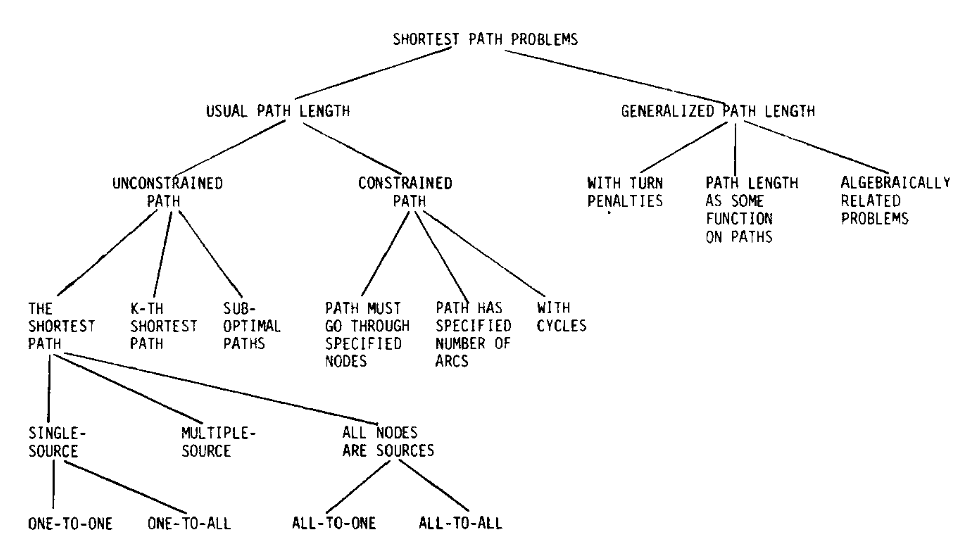
\includegraphics[width=\linewidth]{bilder/shortest path variants tree (Shortest-path algorithms Taxonomy and annotation).png}
	\caption{This image shows a conceptual tree of different variations of shortest path algorithms, taken from \textit{Shortest-path algorithms: Taxonomy and annotation} \cite{deo_shortest-path_1984}}
	\label{fig:shortestPathTaxonomy}	
\end{figure}

Since the shortest path problem has been well-studied and continues to advance in terms of the quality of the returned paths as well as in optimizing the run time of algorithms, the number of approaches to solve this problem is enormous.
The presented tree offers a systematic approach to classify problems of which most fall into one of two categories: they are either single-source shortest paths (SSSP, on the leftmost branch the two bottom-left items) or all-pairs shortest paths (APSP, on the leftmost branch the two bottom-right items).

\paragraph{SSSP}

The first approach -- SSSP -- uses a single starting point and aims to find the shortest path between this point and one or all other vertices.
These problems are commonly encountered in many everyday routing scenarios. 
One-to-one paths, which involve finding the shortest path to a specified destination, have already been discussed in this chapter's introduction (see Section \ref{chapter:introduction}) \cite{sanders_shortest_2019}.
One-to-all paths can be useful for cases like fire departments or the police, which may need a map of the quickest routes to every place in their jurisdiction \cite{sanders_shortest_2019}.

\paragraph{APSP}

The second category aims to find the shortest paths between all vertices in a graph -- either from a specified vertex or from every vertex to every other vertex. 
This calculation of all paths is essential for transportation networks and similar use cases. 
All-to-one path calculations can be useful in scenarios where, following an accident, the nearest of all available emergency vehicles -- with the shortest path -- needs to be determined \cite{khamayseh_efficient_2015}.
For all-to-all paths, many traffic-load calculation problems arise, such as distributing trains along the rail network \cite{curtis_rewire_2012}.


Which of these shortest path algorithms performs best typically depends on the type of graph the implementation is used on, the graphs structure, and the specific problem to be solved. 
A graph can be categorized in different ways: planar or non-planar, directed or undirected, weighted or unweighted, and containing only non-negative weights or allowing negative ones as well.
They also can contain cycles or be acyclic, among other categorizations. 
These different types determine which approaches can be applied and which will yield better results.
Some algorithms like Dijkstra can only be used on a specific type of graph without modifications. 
In this case, the graph needs to contain only non-negative edges.
Others are modified versions, specifically designed to handle issues like graphs with negative edges. 


\section{Heuristic Approaches}
\label{sec:metaHeuristics}

In contrast to exact approaches, heuristics do not guarantee for optimal outcomes but can instead improve the runtime of an algorithm.
A heuristic is a technique that is based on experience or statistical insights, specifically focusing on the structure of individual problems \cite{gendreau_handbook_2010}.
The downside of using such an approach is that there is no longer a guarantee to calculate the global optimum, as heuristics mostly find only partial or approximate solutions to a given problem. 
In many cases where exact algorithms would take too much time or space to find the optimal solution, heuristics can be used to find the best possible solution within the given constraints.
For heuristics, several different ideas have been developed, which can be categorized into construction heuristics, improvement heuristics, and metaheuristics \cite{laporte_5_2002,ropke_heuristic_2005}.
However, differentiating between these types is not always trivial and the distinctions are often blurred.

Construction heuristics build their solution from a starting point until a certain boundary is reached. 
They typically do not have a separate improvement phase.
Improvement heuristics aim to enhance an already existing solution.
They perform improvement steps repeatedly until a specified boundary is met, such as a time limit or reaching the threshold for a good enough approximation.
(Iterative) Local Search and Neighborhoods are examples of improvement heuristics that can be used to reach a more optimized solution.

Metaheuristics are a type of heuristic approaches that also seeks to find an approximate solution to a problem that is as optimal as possible.
The distinction between classical heuristics and metaheuristics is that the latter are less tailored to specific problems.
Metaheuristics typically treat a problem as a black box and do not use distinct structures to solve a problem.
On the contrary, a metaheuristic is typically more generalized and can be used to solve several types of problems.
These strategies are used to enable the metaheuristics to not only produce solutions that are locally optimal, but to broaden the search space they can use for finding optima.

Classical heuristics often carry the inherent risk of finding only a local optimum, which may be far from the global one.
To mitigate this risk, higher-level approaches are necessary.
These methods can include using multiple neighborhood structures to broaden the search space, like Simulated Annealing does, or using entirely new concepts like the Ant Colony approach or Genetic Algorithms. 
The metaheuristic ideas used in this thesis will be explained in the following subsections.



\subsection{Ant Colony}
\label{subsec:antColonyBackground}

Ant Colony is a metaheuristic approach that is inspired by the behavior of biological ants, their colonies, and how they search for food.
Real ants start by leaving their nests and walking around randomly. 
When they discover a food source, they pick up the food and return to their nest.
On their way back, they distribute a substance called \textit{pheromone}, which can then be detected by other ants, indicating that a path leads to a potentially good food source. 
Other ants are then more likely to follow a path with more pheromone placed on the respective edges and will, in turn, lay down their pheromone as well, leading to an accumulation of the pheromone on good paths.
Over time the pheromone dissipates and, if not renewed, will eventually evaporate completely, reducing the attractiveness of the corresponding path \cite{dorigo_ant_1996, gendreau_handbook_2010}. 

Furthermore, pheromone distribution inherently leads to using shorter paths. 
When several ants have to choose between paths, they will first select at random.
However, once an ant discovers the food source, returns to the nest and distributes pheromone along the way back, this process automatically increases the likelihood of the respective path being taken by other ants.
Shorter paths will receive more pheromone as the returning ants will be quicker, leading to a faster distribution of pheromone.
Consequently, more ants will choose this shorter path and thus deposit even more pheromone on it, leading to a self-reinforcing loop that converges when all ants choose the best path only.
Eventually, the pheromone on all paths that are not as good (i.e. longer) will evaporate over time, leaving the best route as the only remaining option \cite{dorigo_ant_1996, gendreau_handbook_2010}.

To illustrate pheromone distribution, Figure \ref{fig:antSystemExampleIllustration} shows how real ants find food and establish a good path to the source. 
In part \textbf{(a)} on the left side, there are many ants moving between two points, A and E, which could represent the nest and a food source.
In part \textbf{(b)} in the middle, an obstacle has been added.
This construction now gives the ants a choice of which path to follow. 
Initially, the likelihood of choosing either path is around 50\%.
While taking the path, the ants distribute pheromone on it. 
On the shorter route, the ants will reach the food source earlier, thus returning quicker than those who took the long path and distribute more pheromone on the shorter path.
For the first few ants, there will be almost no change in the attractiveness of either path.
However, as more ants take the shorter route and return quicker, more pheromone will accumulate on that path.
This increased pheromone concentration leads to a shift in attractiveness, making the shorter path more attractive and more likely to be chosen by later ants, as shown in \textbf{(c)} on the right side.
These ants will, in turn, again increase the amount of pheromone placed, making the path even more attractive.
Thus, the ants create a self-reinforcing loop of positive feedback through their pheromone, which eventually leads to a state where all ants constantly choose the shorter path.


\begin{figure}
	\begin{centering}
		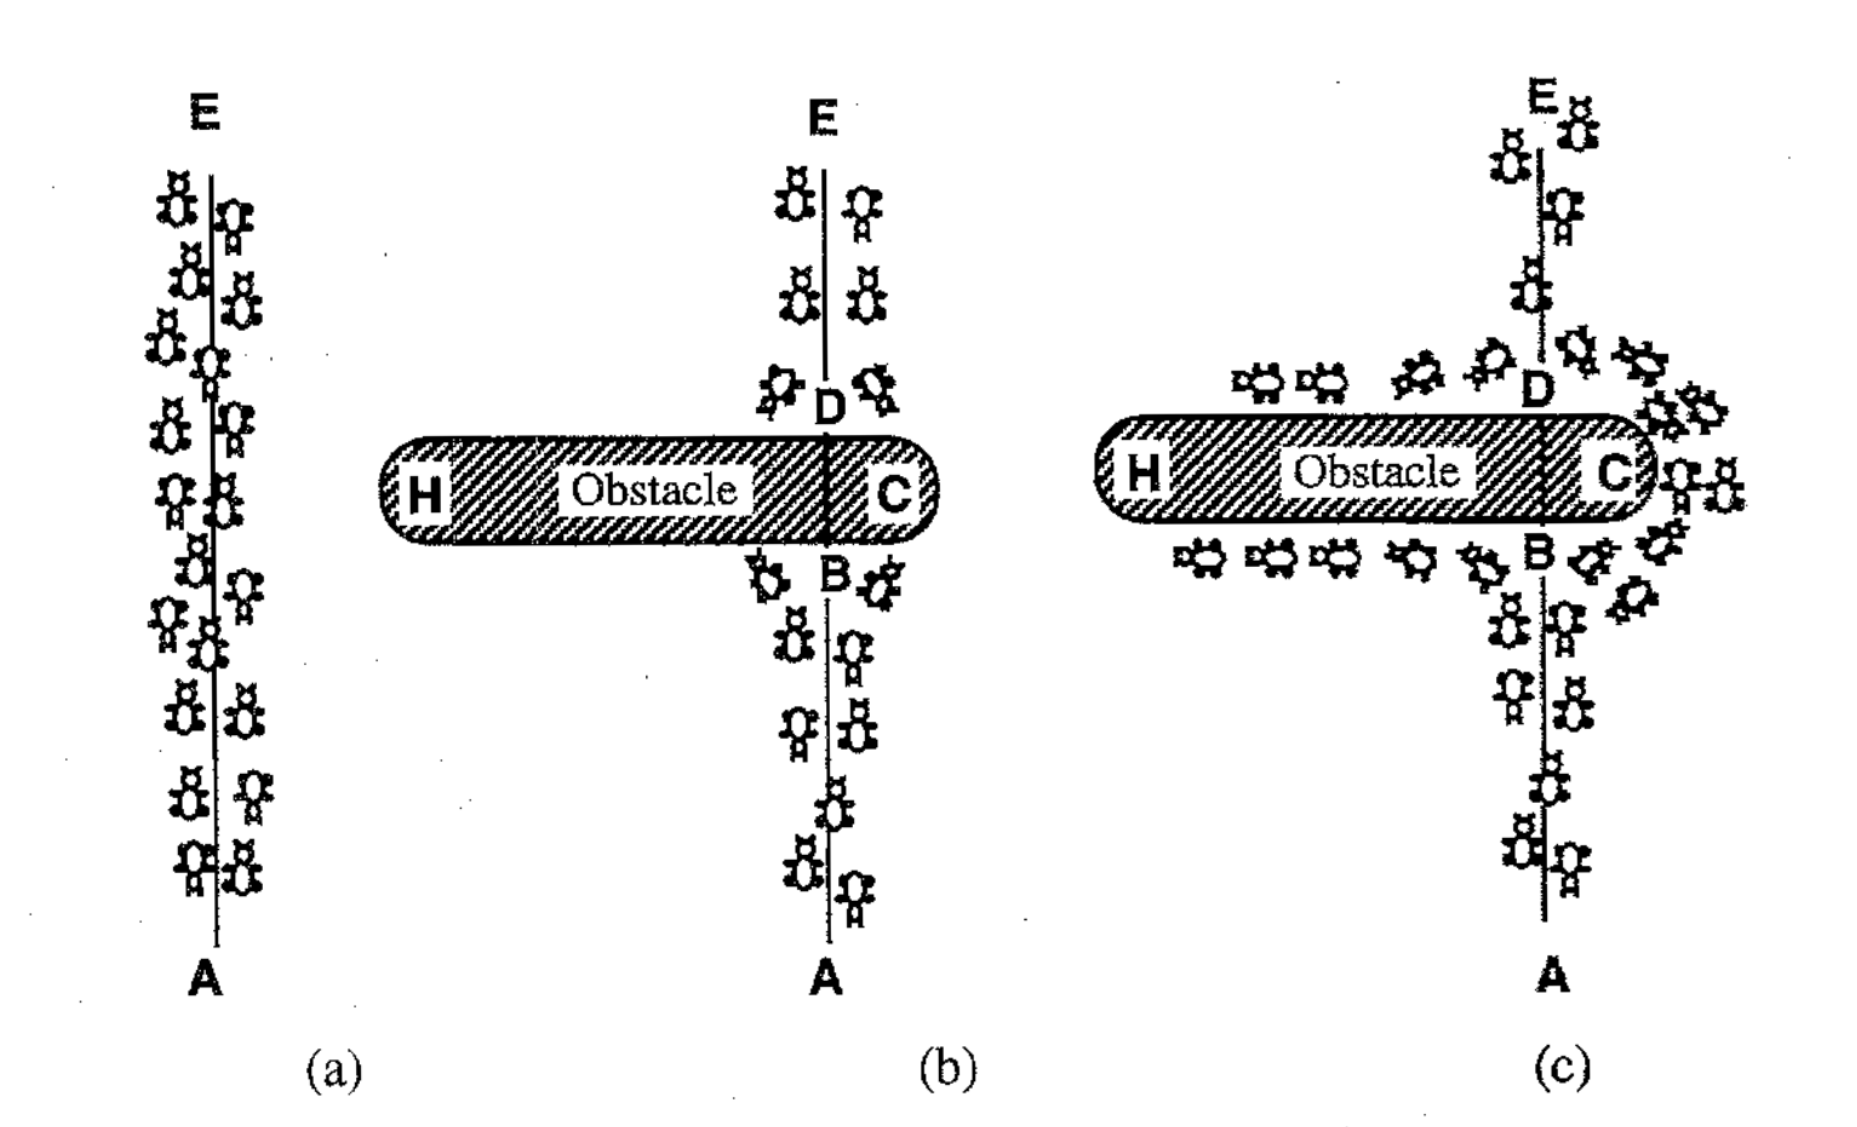
\includegraphics[width=0.8\textwidth]{bilder/antSystemExampleIllustration.png}
		\caption{This figure shows an example of pheromone distribution with real ants. Taken from \textit{Ant System: An Optimization by a Colony of Cooperating Ants} \cite{dorigo_ant_1996}}
		\label{fig:antSystemExampleIllustration}
	\end{centering}
\end{figure}


This behavior can be replicated in virtual graphs for various routing problems.
Ant System has been first introduced in 1990 by Dorigo et al.\ \cite{dorigo_ant_1996} and the following explanations about calculations are based on their findings.
In their paper, the authors describe how to use ants for solving the TSP.
This problem is different from the question of finding a roundtrip with a certain length (plus additional user preferences).
However, in the paper, they stress the adaptability of Ant System approaches, showing both versatility and robustness on different example problems.


\subsubsection{Calculations}
\label{subsubsec:antCalculations}

To transform the analogy of real ants into an algorithm, some formulas and calculations are needed.
Ants are very simple agents. 
They can only do two things:
pick the next node to move to and place pheromone on a path.
They communicate with other ant agents through the pheromone trails, making this process a decentralized way of communication without the need for a central agent.
For the algorithm, a set number of $m$ ants move through the graph, try to find a good route, and place pheromone on edges.
Every ant has a defined amount of pheromone to place. 
How much of the pheromone will be laid on a path ($\Delta\tau_{ij}^k$) can be calculated in several different ways.
Here, $\Delta\tau$ describes the pheromone distribution, while the indices $ij$ indicate the edge where the pheromone is to be placed and $k$ indexes the respective ant.
The authors propose the following three ideas:

\begin{equation}\label{eq:antCycle}
	\Delta\tau_{ij}^k = \begin{cases}
			\frac{Q}{L_k} &\text{if $(i,j) \in$ tour described by $\texttt{tabu}_k(1)$} \\
			0 &\text{otherwise}
	\end{cases}	
\end{equation}


\begin{equation}\label{eq:antDensity}
	\Delta\tau_{ij}^k = \begin{cases}
	Q &\text{if the k-th ant goes from i to j between time} \\
	&\text{t to t+1} \\
	0 &\text{otherwise}
\end{cases}	
\end{equation}


\begin{equation}\label{eq:antQuantity}
	\Delta\tau_{ij}^k = \begin{cases}
	\frac{Q}{c_{ij}} &\text{if the k-th ant goes from i to j between time} \\
		&\text{to t+1} \\\
	0 &\text{otherwise}
\end{cases}	
\end{equation}

Equation \ref{eq:antCycle} is the default formula used by the authors for solving the TSP.
The constant $Q$ must be chosen according to the problem in question.
The variable $L_k$ describes the length of the entire tour created by the k-th ant.
This property is useful for the TSP setting, but is relatively meaningless for tours with a fixed length, as it remains the same value for every ant and every run made.
In cases, where the user defines the length of the tour, $L_k$ will only scale the values chosen for $Q$.
The \texttt{tabuList} contains all nodes that are not allowed to be visited.

Equation \ref{eq:antDensity} uses only the constant Q to describe pheromone placement, without considering the full tour length or individual edge costs. 
Pheromone is placed evenly on all edges, making this method equivalent to an unscaled version of Equation \ref{eq:antCycle} for a fixed length tour.

The last Equation \ref{eq:antQuantity} divides the constant by the length, i.e. the cost of each edge ($c_{ij}$). 
This division reduces the amount of pheromone placed on longer edges compared to shorter edges. 
Although this equation is not influenced directly by the fixed length, this property may still be less useful for tours with a specified length than for TSP.
Since tours that are meant to cover a fixed distance differ from the TSP, where the goal is to find a shortest path that visits all selected cities, Equation \ref{eq:antQuantity} seems the least promising candidate for effective pheromone distribution.

The calculation and placement of pheromone can be defined with different formulas depending on the problem and the optimization goal. 
A suitable option will be detailed in the implementation Chapter (\ref{chapter:implementedChanges}).


Applying a suitable formula to calculate the pheromone distribution, this value can then be used to calculate the overall distributed pheromone for each edge $(i,j)$ that was placed by all ants during one iteration.
This value is described by $\Delta\tau_{ij}$ as follows:

\begin{equation}\label{eq:deltaTau}
	\Delta\tau_{ij} = \sum_{k=1}^{m} \Delta\tau_{ij}^k 
\end{equation}

\paragraph{Trail Intensity Calculation}

This overall value can then be employed to calculate the so called \textit{intensity} of the placed pheromone trail.
Since pheromone evaporates over time, this property has to be modeled as well, using a new parameter $\rho$, which describes how much of the pheromone stays on the trail between two time steps.
Thus, the overall pheromone intensity can be described by

\begin{equation}\label{eq:trailIntensity}
	\tau_{ij}(t+n) = \rho \cdot \tau_{ij}(t)+\Delta\tau_{ij}^k 
\end{equation}

where $\tau_{ij}(t)$ is the previous pheromone intensity and $t+n$ describes the next time step after one full tour was created in $n$ steps.

Using these calculations, the pheromone intensity on all paths can be represented. 
The next step is to determine the probability with which ants will choose a certain edge over other options.
For this calculation, two more properties are needed: the visibility of an edge and the tabuList, containing not-allowed nodes.

\paragraph{Visibility and Transition Probability Calculation}

The tabuList collects all nodes that have been visited before, ensuring that no node is visited more than once, which is necessary for round trips to remain circular rather than repeating the same path in both directions.
In Chapter \ref{chapter:evaluation}, various configurations are tested to represent different shapes and allow for more  user-defined options. 
Thus, for other shapes, this list is not needed.
For the TSP-case, the visibility $\nu_{ij}^k$ is calculated using the cost $c_{ij}$ of the edge $(i,j)$ as follows:

\begin{equation}\label{eq:visibility}
	\nu_{ij}^k = \frac{1}{c_{ij}}
\end{equation}

and the transition probability is given by

\begin{equation}\label{eq:transitionProbability}
	p_{ij}^k = \begin{cases}
		\frac{[\tau_{ij}(t)]^{\alpha} \cdot [\nu_{ij}]^{\beta}}{\sum_{k \in \texttt{allowed}_k} [\tau_{ij}(t)]^{\alpha} \cdot [\nu_{ij}]^{\beta}} &\text{if $j \in \texttt{allowed}_k$ }\\
		0 &\text{otherwise}
	\end{cases}
\end{equation}

using all previously defined values to calculate visibility $\nu_{ij}^k$, trail intensity $\tau_{ij}$, pheromone distribution per ant  $\Delta\tau_{ij}^k$ and overall $\Delta\tau_{ij}$.
Here, $\alpha$ and $\beta$ are parameters that influence the weight of trail intensity and visibility respectively.
Higher values of $\alpha$ increase the significance of the pheromone on the trail (setting $\alpha$ to 0 would lead to completely ignoring the pheromone placed), and higher values of $\beta$ increase the importance of the visibility of an edge (making longer edges less attractive when using the given visibility calculation for TSP).
These parameters will be experimented with and their influence will be evaluated in Chapter \ref{chapter:evaluation}.
For the visibility, a calculation that is suitable to the AOP is determined in Section \ref{subsec:antColonyImplementation}.

In their paper, Dorigo et al. suggest picking middling values for $\alpha$ and $\beta$ in the range of $[0.5,5]$.
They further stated that the best tour was achieved using $\rho = 0.5$ and $Q=100$.
Overall, the results of experimenting with different parameter configurations showed that for very high or very low values of $\alpha$, no good results could be generated.


Some of these equations must be adjusted and fitted to the given \texttt{Arc Orienteering Problem} (see Section \ref{sec:aop}). 
The adjusted calculations and explanations of the changes made can be found in Section \ref{subsec:antColonyImplementation}.


\subsubsection{Algorithm details}
\label{subsubsec:antPseudocode}

A possible structure for an Ant Colony algorithm is displayed in listing \ref{alg:AntColony}, based on the original framework provided in \cite{dorigo_ant_1996}.
Therefore, all formulas are centered around the shortest path that connects all cities in the graph.
Here, the tabuList is used to track all visited cities, the probability is calculated using Equation \ref{eq:transitionProbability}. 
The variables \texttt{NC} and $\texttt{NC}_{MAX}$ are used for the loop count and the maximum number of loops allowed respectively.

In the initialization, the base values are set.
Differences $\Delta\tau_{ij}(t)$ as well as $t$ and \texttt{NC} are set to $0$ while the trail intensity $\tau_{ij}(t)$ is assigned an initial value of $c$.
The ants are placed on a set of cities.
Then, the main loop is started in which the ants are moved according to the probability.
All visited towns are appended to the tabuList, which is full once all cities are added.
This step completes one tour for all ants.

The next steps are necessary to reset and recalculate the needed values for the next run.
In the loop, the ants are moved back to their starting positions, the length of their respective tours is calculated and with it the pheromone that is to be placed on the edge ($\Delta\tau_{ij}^k$) for the current ant $k$.
Using this pheromone, the final pheromone distribution for all ants ($\Delta\tau_{ij}$) is updated.
Furthermore, the new shortest tour, if a better one was found, is updated.
After the individual pheromone values are updated, the trail intensity $\tau_{ij}(t+n)$ has to be recalculated. 
For this step, the evaporation rate $\rho$ scales the current trail intensity and the calculated resulting pheromone for all ants ($\Delta\tau_{ij}$) are added.

The rest of the loop is updating the loop count \texttt{NC}, the time step $t$, and resetting the pheromone for each edge to the initial $0$.
The loop is continued with emptied \texttt{tabuList} if the maximum count was not reached and is ended otherwise, returning the shortest tour found.






\subsection{Simulated Annealing}
\label{subsec:simulatedAnnealingBackground}

Simulated Annealing (SA) builds upon the statistical physics concept of annealing.
The physical process of annealing describes a thermal procedure to improve solids.
Improving in this case means \enquote{obtaining low energy states of a solid in a heat bath} \cite{aarts_simulated_2005}.
Low energy is needed to achieve the stable solid state of a crystal \cite{delahaye_simulated_2019} (see Figure \ref{fig:annealingIllustration} for a visualization of the different states).

The physical process is split into two general steps:
\begin{itemize}
	\item Heating the solid until the atoms can move more freely
	\item Cooling the material to a specified temperature
\end{itemize}
The basic concept is that, given a sufficiently high starting temperature to which the material is heated and a long enough cooling time, the material can reach a stable solid state. 

\begin{figure}
	\centering
	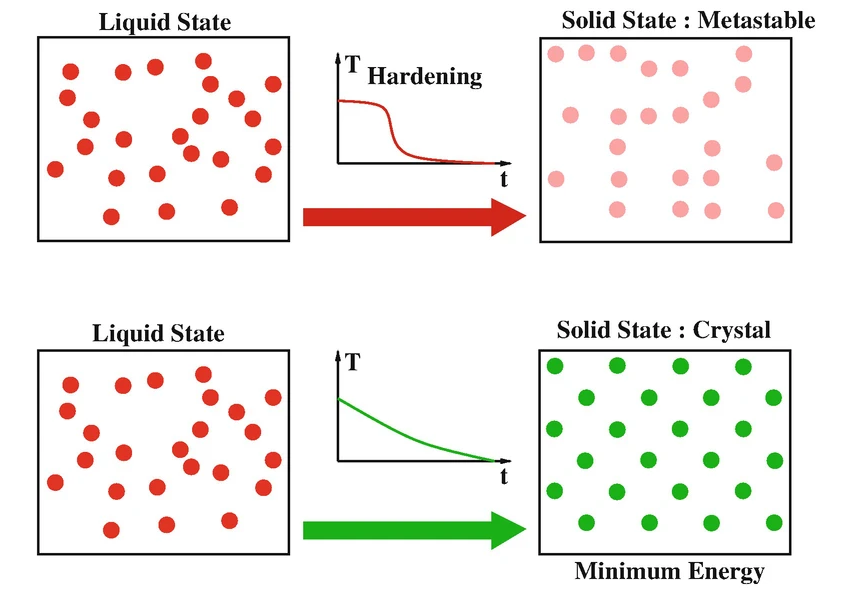
\includegraphics[width=0.9\textwidth]{bilder/AnnealingIllustration.png}
	\caption{The illustration shows two different cooling procedures for a material. The upper one depicts the effects of sudden cooling, resulting in a meta-stable state, while the lower one portrays a slower cooling schedule, which results in a stable solid state. Taken from \textit{Simulated Annealing: From Basics to Applications} \cite{delahaye_simulated_2019}.}
	\label{fig:annealingIllustration}
\end{figure}


Figure \ref{fig:annealingIllustration} shows the effects of different cooling schedules on a material and the type of solid state this material will obtain as a result.
The top-left image shows a liquid state, in which molecules are free and can move around.
Cooling down quickly hinders the atoms from moving into proper positions, resulting in an unordered, non-symmetrical state, which is meta-stable (top-right).
In contrast, the lower part depicts a slower cooling process, where the atoms are given enough time to move into symmetrical form (bottom-right).
This state is equivalent to a minimum energy state, resulting in a stable crystal structure and a highly durable solid material. 
%\# TODO check this! This is not fully correct


Based on this analogy, SA was developed as a concept to solve NP-hard computational problems by improving local search variants \cite{aarts_simulated_2005, eglese_simulated_1990}.
Local search approaches are good at finding locally optimal solutions, but can easily fail to find a global optimum.
SA addresses this problem with the underlying idea based on the two steps of heating and slow cooling.
The distinguishing feature of SA is that the algorithm permits the acceptance of solutions with a certain probability (temperature) that may be inferior to the optimal solution.


\paragraph{Basic Structure of SA}

First, a basic solution for the problem is needed.
For the use case of this thesis, a basic solution is a roundtrip.
Furthermore, a function that determines the quality of the solution is needed, so that comparing different solutions becomes possible. 
Starting from the initial roundtrip, neighboring solutions need to be generated and their quality will be assessed using the quality function.
Any neighboring roundtrip that yields a better result will be accepted as the new solution that has to be improved.
Worse roundtrips can also be accepted based on a cooling schedule.

The schedule contains an initial temperature and a function to calculate the cooling of this value, gradually reducing the temperature over time.
In the beginning, the solution is likely to be further away from a global optimum.
Therefore, a higher temperature allows for an increased likelihood of accepting solutions with a lower quality, which in turn allows for escaping local optima.
As SA progresses, the temperature decreases, reducing the likelihood of accepting inferior solutions as the algorithm approaches the global optimum. 
Achieving this global optimum requires several nested runs:
an outer loop updates the temperature with lower values while an inner loop tests several possible neighborhoods for each temperature state. 
Solutions that are better than the previous one are always chosen, while solutions that are worse than the previous one are selected based on the temperature.


For SA to yield a good result, several parameters need to be established. 
First, a starting roundtrip is calculated to create the baseline.
Then, the initial temperature and the cooling formula are determined.
Furthermore, a neighboring roundtrip has to be identified, along with a formula to assess the quality of all solutions found.
The number of runs is also decided, while both the runtime and the quality of the resulting tour are taken into account.

For some parameters, such as the initial temperature and the cooling formula, thorough testing of different configurations is necessary.
For others, only a limited set of options is relevant.
Determining a neighboring roundtrip as well as an initial solution are parameters with a wide array of calculation possibilities:
Any viable algorithm can be chosen to calculate the initial solution. 
For this thesis, the choice is detailed in Section \ref{subsec:simulatedAnnealingImplementation}.
To determine a neighboring solution, there are a few options that can yield good results.
One approach is to randomly select two vertices and switch their position in different ways within the roundtrip path or variations of this idea \cite{zhan_list-based_2016}. 
Again, the operation chosen for this thesis is described in Section \ref{subsec:simulatedAnnealingImplementation}.



%For an initial solution, the implemented algorithms -- AntColony, Greedy and MinCost (see \ref{subsec:Tour4Me}) -- can calculate a base roundtrip.
%Which of these is the preferred depends on the preferences of the resulting shape. 
%Greedy and AntColony prioritize edge quality, while MinCost primarily optimizes for a rounder shape.
%
%Another approach is to create waypoints, similar to how it is done in the MinCost algorithm but without the length restrictions.
%The generated initial solution can then be used to generate a set of waypoints. 
%Based on this node set, neighboring roundtrips are ones where the tour is modified by removing, adding, or moving one of the waypoints.

%
%To remove a waypoint, the node and the paths connecting this vertex to the two neighboring waypoints need to be deleted. 
%The two ends are then reconnected using either a shortest path or a MinCost approach.
%To add a waypoint, a suitable node needs to be determined, first. 
%This choice can be done either randomly or based on a probability distribution that gives higher probabilities to nodes closer to the path and decreases in value the further away a node is.
%Once a suitable node is chosen, the closest waypoint and the best neighbor needs to be identified.
%This selection is done by calculating the shortest paths from the new waypoint to all existing waypoints.
%The connection between the two selected nodes is then removed, and the new waypoint is connected to the two nodes that now frame the gap. 
%Moving a waypoint involves both removal and addition:
%First, the new node is found, and then the closest waypoint is removed.
%



\subsubsection{Calculations}
\label{subsubsec:SACalculations}

For SA, several parameters need to be calculated.
First, the initial temperature and the respective cooling schedule or a function to decrease the value have to be determined.
Various functions can be applied, provided that they decrease the temperature and are suited to the problem.
For example, a simple function that calculates the temperature by using the difference between the quality of the neighboring solution $f(j)$ and the quality of the current solution $f(i)$, divided by the natural logarithm of a random number $r_i$ \cite{zhan_list-based_2016}: 

\begin{equation}\label{eq:temperatureSchedule}
	T_{i+1} = \frac{- |f(j)-f(i)|}{ln(r_i)}	
\end{equation}

In this equation, $r_i$ is smaller than a previously calculated probability $p_i$.
Only when $r_i$ was smaller, the respective solution with a worse quality is accepted. 
The probability $p_i$ is calculated using the difference between the quality of the neighboring solution $f(j)$ and the quality of the current solution $f(i)$, divided by the maximum temperature as exponents of the euclidean function: 
$p_i = e^{\frac{- |f(j)-f(i)|}{t_{max}}}$ \cite{zhan_list-based_2016}.

Another option is to multiply the current temperature by a factor $\alpha$ smaller than 1 \cite{eglese_simulated_1990}:

\begin{equation}\label{eq:temperatureSchedule2}
	T_{i+1} = \alpha \cdot T_i
\end{equation}

Or scaling by using a constant $b$ to form a fraction \cite{eglese_simulated_1990}: 
\begin{equation}\label{eq:temperatureSchedule3}
	T_{i+1} = \frac{T_i}{1 + b \cdot T_i}	
\end{equation}

Several other options exist, as listed in the paper by R. W. Eglese \cite{eglese_simulated_1990}, to calculate the temperature, where the key criterion is that the temperature decreases over time.

The quality function $f$ is highly dependent on the problem at hand and thus can vary significantly. 
For the TSP, the quality of a tour is determined by the respective length.
For the AOP, the quality is determined by the values that are to be collected when generating a roundtrip. 
How the quality is calculated for the specific case in this thesis is described in detail in Section \ref{subsec:simulatedAnnealingImplementation}.

Another important calculation is the probability of accepting a worse solution.
This probability can be determined by using the temperature and the quality values of the two solutions \cite{eglese_simulated_1990}.
The difference between the quality of the neighboring solution $f(j)$ and the current solution $f(i)$ is always negative, because a positive difference implies $f(j) > f(i)$, resulting in the neighboring solution being chosen automatically.
Since the probability is calculated only when the difference is negative, the exponent will always be less than $1$, resulting in a valid probability function that has a value closer to 1 when the difference is small, and closer to $0$ when this difference is large.


\begin{equation}\label{eq:SAprobCalculation}
	p = e^{\frac{f(j)-f(i)}{T}}
\end{equation}



\subsubsection{Algorithm details}
\label{subsubsec:SAPseudocode}

The SA algorithm has a basic structure that remains consistent across different problems.
This structure is outlined in the pseudocode in \ref{alg:SApseudocode}, based on Eglese \cite{eglese_simulated_1990} and Zhan et al.\ \cite{zhan_list-based_2016}. % and visualized in a flowchart diagram in Figure \ref{fig:SAFlowchart}.

First, an initial roundtrip has to be determined. 
This calculation can be performed using any algorithm that produces a valid solution, such as a Greedy approach or the MinCost algorithm, which is also used for solving the AOP in the original Tour4Me application (see Section \ref{subsec:Tour4Me}).
Furthermore, a starting temperature must be set, which will be used for the initial probability calculations and then decreased after the iterations of the inner loop.

Next, the two loops of the main SA step are executed.
The outer loop is bound by a selectable number of runs, while the inner loop is bound by a selectable number of repetitions that should be performed with a fixed temperature.
The outer loop controls how many new temperatures are tested -- in the physics analogy, this property equates to how long the material is left to cool -- with decreasing temperatures.
The inner loop controls the number of attempts made before the temperature is adjusted. 
Alternatively, the outer loop can use reaching a certain quality value or a maximum run time as the stopping condition.
Performing several calculations in the inner loop with the same temperature can increase the probability of finding a better solution for the set temperature, as well as the likelihood of choosing a solution with a worse quality.






